\chapter{Pipeline isolation} \label{chapter6}
\minitoc
\eject

The previous chapter presented a compiler to identify and extract the underlying pipeline in a Javascript application.
However, the stages doesn't enforce the isolation required for parallel execution.
Moreover, the Dues that constitues the stages of this pipeline 

only parts of the pipeline are identified, 
This chapter present the second contribution of this thesis.
The equivalence between a memory shared among all the operations and independent memory for each operation in a pipeline.
It tackles the problems arising from the translation of the global memory synchronization into message passing.

This equivalence is implemented as a compiler, improving upon the previous one.
The compiler transforms a Javascript application into a network of independent parts communicating by message streams and executed in parallel.
We named these parts \textit{fluxions}, by contraction between a flux and a function.
% Fluxions are executed in an execution model that assure parallelism and communications.

% We present an early version of this tool as a proof of concept for this compilation approach.
Section \ref{section:model} describes the execution model that executes fluxions in parallel, and assure their communications.
The compiler, and the equivalence are described in section \ref{section:compiler}.
Section \ref{section:evaluation} a real-case test of compilation, and expose the limits of this compiler.

\section{Fluxional execution model} \label{section:model}

% The compiler we present in section \ref{section:compiler} focuses on web applications that tend to follow the functional paradigm while keeping a global memory.
% Such applications are built using functions that are executed sequentially to assure the exclusivity of access on the global memory.
% This is a serious performance issue, as it avoids to leverage the parallelism of modern architectures.

% We present in this section a different execution model that isolates the memory accessible to some functions.
% This approach allows to execute these functions in parallel, hence, to benefit of the performance improvements of this parallelism.
% This execution model is close to the actor model, as the function are executed on autonomous execution units with their own isolated memory, communicating by messages.

% In this section, we present an execution model to allow the execution of functions in parallel of a main thread.
% Each parallel function is encapsulated in an autonomous execution container with its own memory.

In this section, we present an execution model to provide scalability to web applications.
% The execution of functions may dynamically be reallocated at run time depending on the load of servers.
To achieve this, the execution model provides a granularity of parallelism at the function level.
Functions are encapsulated in autonomous execution containers with their state, so as to be reallocated and executed in parallel.
This execution model is close to the actors model, as the execution containers are independent and communicate by messages.
The communications are assimilated to stream of messages, similarly to the dataflow programming model.
It allows to reason on the throughput of these streams, and to react to load increases.
% As we focus on real-time web applications, the streams of message correspond to the input stream of requests.

% This execution model is also close to the functional paradigm, as the execution container contains function to execute at each message reception.
% The function receives parameters from the input message, and sends one, or more, output streams of messages to other execution container.

The fluxional execution model executes programs written in our high-level fluxional language, whose grammar is presented in figure \ref{fig:flx-lang}.
An application $\bnfpn{program}$ is partitioned into parts encapsulated in autonomous execution containers named \textit{fluxions} $\bnfpn{flx}$.
In the following paragraphs, we present the \textit{fluxions}.
Then we present the messaging system to carry the communications between \textit{fluxions}.
Finally, we present an example application using this execution model.

\subsection{Fluxions}
% $\bnfpn{flx}$
% $\bnfpn{id}$
% $\bnfpn{fn}$
% $\bnfpn{ctx}$
% $\bnfpn{fn}$
% $\bnfpn{stream}$
% $\bnfpn{dest}$

% The fluxional execution model manages and invokes fluxions.
A \textit{fluxion} $\bnfpn{flx}$ is named by a unique identifier $\bnfpn{id}$ to receive messages, and might be part of one or more groups indicated by tags $\bnfpn{tags}$.
A \textit{fluxion} is composed of a processing function $\bnfpn{fn}$, and a local memory called a \textit{context} $\bnfpn{ctx}$.
% Figure \ref{fig:flx-lang} presents the fluxional language we designed to express fluxions.
% The function encapsulated by a \textit{fluxion} consumes an input stream and generates one or more outputs streams.
At a message reception, the \textit{fluxion} modifies its \textit{context}, and sends messages on its output streams $\bnfpn{streams}$ to downstream \textit{fluxions}.
The \textit{context} handles the state on which a \textit{fluxion} relies between two message receptions.
% A message is composed of the recipient fluxions' names and a body.
% Message passing is unable\footnote{at reasonable costs} to replace the synchronization allowed by shared state. % and required between some of the application parts.
In addition to message passing, the execution model allows \textit{fluxions} to communicate by sharing state between their \textit{contexts}.
% To allow this synchronization when required, the execution model allows fluxions to share state between their contexts.
The fluxions that need to synchronize together are grouped with the same tag, and loose their independence.
% To assure the consistency of the shared state, all the fluxions of a group are executed sequentially.
% Though, the different groups of fluxions are executed in parallel.

There are two types of streams, \textit{start} and \textit{post}, which correspond to the nature of the rupture point yielding the stream.
We differentiate the two types with two different arrows, double arrow (\texttt{>>}) for \textit{start} rupture points and simple arrow (\texttt{->}) for \textit{post} rupture points.
%We differentiates the two types with two different arrows, double arrow ($\twoheadrightarrow$ or \texttt{>>}) for \textit{start} rupture points and simple arrow ($\to$ or \texttt{->}) for \textit{post} rupture points.
The two types of rupture points are further detailed in section \ref{section:compiler:analyzer:rupture}.


% Fluxions are executed on an event-loop with an isolated heap ; it is a \textit{Node.js} instance.
% We propose to stretch the execution of an application by distributing the fluxions on different event-loops.
% But the distribution is limited by the dependencies between fluxions.
% All the fluxions of a group need to be gathered on the same event-loop.
% Indeed, each event-loop assures the exclusivity of access to the state: only one fluxion is executed at once.
% Consequently, the more fluxions are gathered on an event-loop, the less time fraction each fluxion can use without impacting the throughput.

%These groups represent the graph of state communications between fluxion.
%Hence, this graph indicates the states that are limiting the parallelism.


% A fluxion receiving and sending heap reference can be stateless, hence replicated.
% However, because it share references, it needs to be on the same group than other another fluxions (think about req / res).
% If all the fluxion of a group are stateless, they can be replicated exactly like if it was a single fluxion. 








% It is the target for our compiler.
\begin{figure}
\vspace{-0.6\baselineskip}
\begin{bnf*}
  \bnfprod{program}    {\bnfpn{flx} \bnfor \bnfpn{flx} \bnfsp \bnftd{eol} \bnfsp \bnfpn{program}}\\
  \bnfprod{flx}        {\bnfts{\texttt{flx}} \bnfsp \bnfpn{id} \bnfsp \bnfpn{tags} \bnfsp \bnfpn{ctx} \bnfsp \bnftd{eol} \bnfsp \bnfpn{streams} \bnfsp \bnftd{eol} \bnfsp \bnfpn{fn}}\\
  % \bnfprod{tags}       {\bnfts{\bnfpn{id}} \bnfor \bnfpn{id} \bnfsp \bnftd{eol} \bnfsp \bnfpn{tags} \bnfor \bnftd{empty string}}\\
  \bnfprod{tags}       {\bnfts{\texttt{\&}} \bnfsp \bnfpn{list} \bnfor \bnftd{empty string}}\\
  \bnfprod{streams}    {\bnfts{\texttt{null}} \bnfor \bnfpn{stream} \bnfor \bnfpn{stream} \bnfsp \bnftd{eol} \bnfsp \bnfpn{streams}}\\
  \bnfprod{stream}     {\bnfpn{type} \bnfsp \bnfpn{dest} \bnfsp [\bnfpn{msg}]}\\
  \bnfprod{dest}       {\bnfpn{list}}\\
  \bnfprod{ctx}        {\bnfts{\texttt{\{}} \bnfpn{list} \bnfts{\texttt{\}}}}\\
  \bnfprod{msg}        {\bnfts{\texttt{[}} \bnfpn{list} \bnfts{\texttt{]}}}\\
  \bnfprod{list}       {\bnfpn{id} \bnfor \bnfpn{id} \bnfsp \bnfts{,} \bnfsp \bnfpn{list}}\\
  \bnfprod{type}         {\bnfts{\texttt{>}\texttt{>}} \bnfor \bnfts{\texttt{-}\texttt{>}}}\\
  \bnfprod{id}         {\bnftd{Identifier}}\\
  \bnfprod{fn}         {\bnftd{imperative language and stream syntax}}\\
\end{bnf*}
\vspace{-2.5\baselineskip}
\caption{Syntax of a high-level language to represent a program in the fluxional form}
\label{fig:flx-lang}
\end{figure}

\subsection{Messaging system}

% In a distributed approach, the messages between fluxions would be carried over a distributed message broker.
% However this execution model is only a simulation of a distributed execution environement.
% We simplify the distributed message broker with a master message queue to centralize communication between workers, though, each worker has its own local message queue.
% The messaging system is the core of the execution model.
% It carries messages and invokes fluxions at reception.
% The messaging system sends messages to the worker hosting the destination fluxion.
% Locally, the master worker hosts fluxions that need access to the external network or the global memory.
% Using a message queue allows to execute multiple processing chains fairly and concurrently, without difference in scheduling local messages, or network messages.

The messaging system assures the stream communications between fluxions.
It carries messages based on the names of the recipient fluxions.
After the execution of a fluxion, it queues the resulting messages for the event loop to process.
% The messages are queued for the event-loop to execute the associated fluxions sequentially.

% The execution model allows each group of fluxions to be executed on a remote event-loop.
% Therefore, some messages need to be send to remote event-loops.
% When processing a message, if the destination fluxion is local, the messaging system immediately invokes the fluxion with the message, if it is on a remote event-loop, the messaging system sends the message to be queued on the remote event-loop.



% The messaging system carries messages from one event-loop to the other, and assure that the message is queued on the event-loop executing the destination fluxion.

% If two fluxions share the same name, it would lead to a conflicting situation for the messaging system.

% This registration associates a processing function with a unique name and an initial \textit{context}.
% The registration is done by calling \texttt{register(<name>, <fn>, <context>)}, \circled{1}.
% A fluxion can dynamically register other fluxions

The execution cycle of an example fluxional application is illustrated in figure \ref{fig:MesSys}.
Circles represent registered fluxions.
The source code for this application is in listing \ref{lst:source} and the fluxional code for this application is in listing \ref{lst:fluxional}.
The fluxion \textit{reply} has a context containing the variable \texttt{count} and \texttt{tem\-plate}.
The plain arrows represent the actual message paths in the messaging system, while the dashed arrows between fluxions represent the message streams as seen in the fluxional application.
% The streams between workers are serialized.

% To assure the consistency of their shared contexts, all the fluxions grouped with the same tag are executed sequentially and share the same message queue.
% Though, the different groups of fluxions are executed in parallel with different event queues.

% This first message represents the incoming of a request from a user.
The \textit{main} fluxion is the first fluxion in the flow.
When the application receives a request, this fluxion triggers the flow with a \texttt{start} message containing the request, \circled{2}.
This first message is to be received by the next fluxion \textit{handler}, \circled{3} and \circled{4}.
The fluxion \textit{handler} sends back a message, \circled{5}, to be enqueued, \circled{6}.
The system loops through steps \circled{3} through \circled{6} until the queue is empty.
This cycle starts again for each new incoming request causing another \texttt{start} message.

\begin{figure}[h!]
  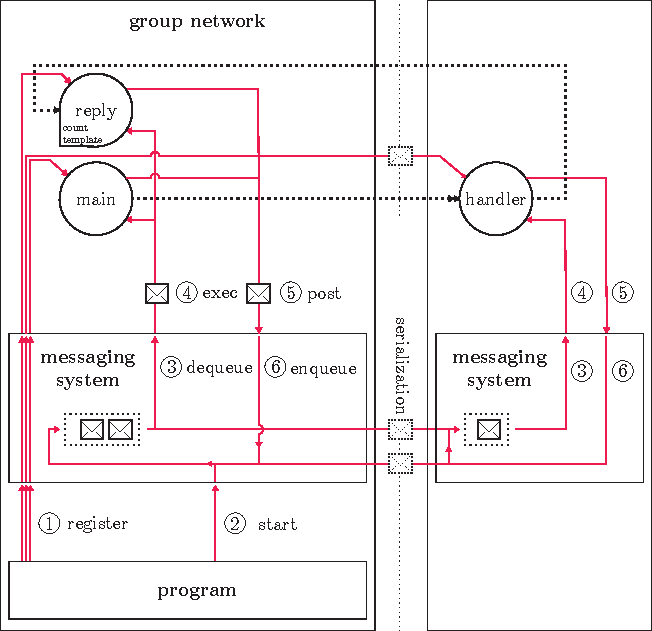
\includegraphics[width=\linewidth]{resources/schema-message.pdf}
  \caption{The fluxional execution model in details}
  \label{fig:MesSys}
\end{figure}

% Algorithms \ref{alg:parcours} and \ref{alg:traitement} describe the behavior of the messaging system after the \texttt{start} function invocation.

% \begin{algorithm}
% \caption{Message queue walking algorithm}
% \label{alg:parcours}
% \begin{algorithmic}
% \Function{loopMessage}{\null}
% \While{$msg$ \textbf{presents in} $msgQueue$}
% \State $msg \gets$ \Call{dequeue}{\null} \Comment{\circled{3}}
% \State \Call{ProcessMsg}{$msg$}
% \EndWhile
% \EndFunction
% \end{algorithmic}
% \end{algorithm}

% \begin{algorithm}
% \caption{Message processing algorithm}
% \label{alg:traitement}
% \begin{algorithmic}
% \Function{processMsg}{$msg$}
% \For{$dest$ \textbf{in} $msg.dest$}
% \State $worker \gets lookup(dest)$
% \State \Call{worker.send}{$fluxion, msg.body$} \Comment{\circled{4}}
% % \State $message \gets$ \Call{exec}{$fluxion, msg.body$} \Comment{\circled{4} \& \circled{5}}
% % \State \Call{enqueue}{$message$} \Comment{\circled{6}}
% \EndFor
% \EndFunction
% \end{algorithmic}
% \end{algorithm}

\subsection{Service example}

To illustrate the fluxional execution model, and the compiler, we present in listing \ref{lst:source} an example of a simple web application.
This application reads a file, and sends it back along with a request counter.

\begin{code}[js,
  caption={Example web application},
  label={lst:source}]
var app = require('express')(),
    fs = require('fs'),
    count = 0;

app.get('/', function handler(req, res){
  fs.readFile(__filename, function reply(err, data) {
    count += 1;
    res.send(err || template(count, data));
  });
});

app.listen(8080);
\end{code}

% The original source code of this application is available in listing \ref{lst:source}\footnote{The listings are also available on github\cite{flx-example}.}.
% In this example application, some points are worth noticing.
The \texttt{handler} function, line 5 to 11, receives the input stream of request.
The \texttt{count} variable at line 3 increments the request counter.
This object needs to be persisted in the fluxion \textit{context}.
The \texttt{template} function formats the output stream to be sent back to the client.
The \texttt{app.get} and \texttt{res.send} functions, respectively line 5 and 8, interface the application with the clients.
And between these two interface functions is a chain of three functions to process the client requests : \texttt{app.get} $\to$ \hspace{-1.4em} $\to$ \texttt{handler} $\to$ \texttt{reply}.
This application is transformed into the high-level fluxional language in listing \ref{lst:fluxional} which is illustred in Figure \ref{fig:MesSys}.
% We expect a similar result with the compiler described in section \ref{section:compiler}.
% Horizontal dashed lines show virtual transmission of messages between fluxions although they all go through the messaging system.

% \begin{figure}[h!]
%   \includegraphics[width=\linewidth]{ressources/flux.pdf}
%   \caption{Fluxions chain manually extracted from the example application}
%   \label{fig:fluxions}
% \end{figure}

\begin{code}[flx, caption={Example application expressed in the high-level fluxional language}, label={lst:fluxional}]
flx main & network
>> handler [res]
  var app = require('express')(),
      fs = require('fs'),
      count = 0;

  app.get('/', >> handler); //@\label{lst:fluxional-streamtohandler}@
  app.listen(8080);

flx handler
-> reply [res]
  function handler(req, res) {
    fs.readFile(__filename, -> reply); //@\label{lst:fluxional-readfile}@
  }

flx reply & network {count, template}
-> null
  function reply(error, data) {
    count += 1; //@\label{lst:fluxional-counter}@
    res.send(err || template(count, data)); //@\label{lst:fluxional-ressend}@
  }
\end{code}

The application is organized as follow.
The flow of requests is received from the clients by the fluxion \texttt{main}, it continues in the fluxion \texttt{handler}, and finally goes through the fluxion \texttt{reply} to be sent back to the clients.
The fluxions \texttt{main} and \texttt{reply} have the tag \texttt{network}.
This tag indicates their dependency over the network interface, because they  received the response from and send it back to the clients.
The fluxion \texttt{handler} doesn't have any dependencies, hence it can be executed in parallel.

The last fluxion, \texttt{reply}, depends on its context to holds the variable \texttt{count} and the function \texttt{template}.
It also depends on the variable \texttt{res} created by the first fluxion, \texttt{main}.
This variable is carried by the stream through the chain of fluxion to the fluxion \texttt{reply} that depends on it.
This variable holds the references to the network sockets.
It is the variable the group \texttt{network} depends on.

Moreover, if the last fluxion, \texttt{reply}, did not relied on the variable \texttt{count}, the group \texttt{network} would be stateless.
The whole group could be replicated as many time as needed. % to cope with the incoming traffic.

This execution model allows to parallelize the execution of an application.
Some parts are arranged in pipeline, like the fluxion \texttt{handler}, some other parts are replicated, as could be the group \texttt{network}.
This parallelization improves the scalability of the application.
Indeed, as a fluxion contains its state and expresses its dependencies, it can be migrated.
It allows to adapt the number of fluxions per core to adjust the resource usage in function of the desired throughput.


% Fluxions with no state could be replicated to make data parallelism, additionally to the pipeline parallelism.

Our goal, as described in the introduction, is not to propose a new programming paradigm with this high-level language but to automate the architecture shift.
We present the compiler to automate this architecture shift in the next section.
% # Explanation of the concept

% ## Turn-based programming.

% (see presentation on Dues)
% -> single-thread, no wait, no block and so on
% Shared heap -> no mutex, no synchronization, so it is good scalability


% Turn-based programming is an event-loop.
% It is the execution of queued events one after the other.
% An event is the association of a callback and a message.
% The callback is a small Javascript Program, designed to process the message.
% During its turn, the callback executes, and can queue events : that is register callback to be executed during a next turn.
% TODO what I mean exactly by queue events ? -> the distinction between the asynchronous operation, and the resulting event.

% ## Pipeline

% So a callback sends messages to other callbacks.
% -> It is exactly like a pipeline.
% However, all the callbacks share the same heap.
% So it is not possible to distribute the different callbacks without synchronization of this heap, or splitting the heap for each callback.
% TODO state VERY clearly this problem, it is at the core of my thesis.

% So, how to split the heap so that each callback has its own exclusive heap ?

\comment{From here, the reader should be confortable with the event-loop, and the analogy we drawn between the event-loop and a pipeline.
The problematic is now clear : how to split the heap so that each asynchronous callback has its own exclusive heap ?}

\section{Callback identification}

\subsection{\comment{TODO}}

\section{Callback isolation}

We explain in this section the compilation process we developped to isolate the memory access for each callbacks.
The result of this process should be two-fold. First each callback should have an exclusive access on a region of the memory. So that two different callback can be executed in parallel. And it should be clear for each callback, what are the variable needed from upstream callbacks, and what are the variable to send downstream.

\subsection{Propagation of variables}


\subsubsection{Scope identification}

In section \ref{??? Javascript scope / closure}, we explained that Javascript is roughly lexically scoped.
A consequence is that the declaration of contexts can be inferred statically.
For example, in a lexically scoped, strongly typed, compiled language, the compiler know the content of each scope during compile time, and can prepare the memory stack to store the variables in each scope.

In most languages, the memory is in two parts : the stack, and the heap.
The stack is statically scoped, and its layout is known at compile time.
The heap, on the other hand is dynamically allocated. Its layout is built at run time.

But Javascript is a dynamic language, perhaps the most dynamic of all languages.
It doesn't have this distinction between stack and heap. Every variable is dynamically allocated on the heap.
That induce two consequences.
The first is that Javascript provides two statements to dynamically modify the lexial scope : \texttt{eval} and \texttt{with}.
The second is that to know the layout of the heap, we need to use static analysis tools.
In the next two sections, we adress these two consequences.

\subsubsection{Break the lexical scope} \label{???:breakscope}

Without these statements, \texttt{eval} and \texttt{with}, Javascript is lexically scoped. It is possible to infer the scope of each variable at compile time.


The \texttt{with} statement continue the execution using an expression as the lexical scope.
As the provided expression is dynamically evaluated, it is possible to dynamically modify the lexical scope.
The code snippet below show an example of such a situation.

\begin{code}
var aliveCat = {isAlive: true};
var deadCat = {isDead: true}

with (Math.random() > 0.5 ? aliveCat : deadCat) {
  isAlive;
  // Half the time -> ReferenceError: isAlive is not defined
  // Half the time -> true;
}
\end{code}

The variable \texttt{isAlive} is defined only in the object \texttt{aliveCat}.
The presence of the variable \texttt{isAlive} in the lexical environment within the \texttt{with} statement cannot be determined statically, as the lexical environment is dynamically linked to either \texttt{aliveCat} or \texttt{deadCat}.

Note that the MDN reference page on \texttt{with}\ftnt{https://developer.mozilla.org/en-US/docs/Web/JavaScript/Reference/Statements/with} says that \textit{Using \texttt{with} is not recommended, and is forbidden in ECMAScript 5 strict mode.}

The \texttt{}

% TODO and specify that Javascript is roughly lexically scoped : it is not completely lexically scoped, and five examples to backup that.

Not to be mistaken with the \texttt{this} operator.
It is possible to dynamically change the content of an object,  
% TODO continue this paragraph about how the this operator change the properties of an object. 
% Does it change the lexical scope, if that object is actually used as a context elsewhere ? -> No, I don't think so.
% But ask on SO, just to be sure.

\begin{code}
function stuff() {
  this.x = 42;
}

stuff.call({})

\end{code}

% Javascript is lexically scoped, therefore we can identify the scope of variable statically.
% (At the exception of eval and with : with is forbidden from strict mode, so that is not a bigdeal, howether, eval is sometimes used in smart ways, but most of the time it is monomorphic (I don't exactly know what that means, I heard from Floreat, it must be something related to PL community)).

% The compiler identifies the variables shared by multiple callbacks from their scope.
% TODO explain this in depth.
% Function scope, closures, and so on ...



However, even if Javascript is lexically scoped, the memory is still dynamicall allocated and manipualeted, so that it is not possible to actually infer the memory layout at compiler time only with lexical scope analysis, and without deeper static analysis.

\subsubsection{Scope Leaking}

% Javascript uses a pass-by-sharing paradigm.
% That means that sometimes the argument of a call are passed by value, sometimes by reference (atomic data type (number, string, bool) -> by value, complex data type (objects) -> by reference).
% That means that the modification of a local variable can affect variable in seemingly unrelated scopes.
% It seems that the points-to analysis is what is used to find stuffs like that (side-effects ?).

% TODO what we are talking about here are aliases.

% TODO I am stating here that in low-level language, the memory access is so fine, that it is difficult to exactly pin down the memory layout in term of object, it is rather seen as a big array of memory adresses.
% While in higher-level language, like Javascript, the memory access is at the property level (it is not possible to access memory down to the adress), so it could be easier (maybe, just not harder) to infer the dynamic memory layout from source.
To infer the layout of the heap at compile time, static analysis tools are used, like the points-to analysis, developped by Andersen in its PhD thesis \cite{Andersen1994}.
For such analysis, the memory is splitted at the access scale.
In low-level languages, like C/C++, the memory is mainly managed by the developer. Allowing access to the memory at a small grained scale : up to the address.
It impose the analysis to split the memory to the adress scale in some cases.
% TODO Backup that, HEAVILY
In higher-level languages, like Javascript, the developer cannot access the memory to the adress scale.
The memory is accessed at a coarser scale : the property scale.
(At the exception of some arrays and buffers, that mimic, and are mapped to actual memory adresses for performance reasons.)
% TODO find exactly the references for these buffers : I think of ArrayBuffer, and sharedArray ... but I am not sure. Need more inspection.

\subsubsection{Propagation of execution and variables}

For the execution of each callback / stage, the corresponding part of the state is local, and the rest is remote, and inaccessible.
We are going to explain why it must remain inaccessible.

While a callback is executing a request, the previous callback (the up stream callback) is executing the next request.
The next request will arrive at the current callback some time in the future.
The modification done in the state of the upstream callback will propagate only later in the current callback.
The state of the upstream callback is in a different time frame than the state of the current callback.

To really understand that, we need to compare this execution with the execution on a unique event-loop.
If the current callback executes, then the upstream callback might have, or might not have started to execute the next request.
But as soon as the current callback executes, the modifications done on the states, are immediatly propagated, so that the upstream callback can take them into account for the next request.

However, if the two callbacks are distant, then the modification of the current callback will not immediatly propagate to the upstream callback.
During the propagation, the upstream callback might execute requests than would not be aware of the state modification from the current callback (from downstream).
That is why we say the upstream callback and the current callback are in two different time frame.
Propagating the state modification upstream is like going backward in time, it is impossible.
That is why the execution, and the state modification propagation must always flow downstream.

As a note, I must add that if an upstream and a downstream callbacks are on the same event-loop, then this doesn't apply. it is like a loop in the time : the modification immediatly propagate from downstream to upstream.






% The execution progress downstream, following the message stream.
% TODO state very clearly this proposition, it is the second core of my thesis (and I love the idea, it relates directly to reality, graivity, and the fabric of the universe <3).

% Because the propagation of the modification is not instantaneous, going back upstream is like going backward in time : it is impossible.
% Therefore, a variable cannot be read upstream a write.
% And it cannot be write downstream either.

% In other words, only one callback can write on a variable -> seems obvious from previous sections.


% In promises, because the heap is not shared, things are less restrictive.
% Multiple stages can read and write the same variable, because the propagation of modification is instantaneous, due to the shared heap.





% TODO write about what it implies to detect continuation in variable, or other expressions.

% Why can we only detect continuations declared in situ.
% If a continuation is passed as a variable, we don't know for sure what is the function associated with, and the closure of that function.

\section{Real case test} \label{section:evaluation}

The goal of this test is to prove the possibility for an application to be compiled into a network of independent parts.
We want to show the current limitations of this isolation and the modifications needed on the application to circumvent these limitations.
% TODO -> and finally, we present the possibilities of future works.
% We want to show the limitations of this isolation for future works, and the modifications needed to circumvent these limitations.

We present a test of our compiler on a real application, gifsockets-server\ftnt{https://github.com/twolfson/gifsockets-server}.
% This application is part of the selection from our previous paper \cite{Brodu2015}.
% We chosed it because it is a working application, simple enough to illustrate this evaluation.
This application was selected from the \texttt{npm} registry because it depends on \texttt{express}, it is tested, working, and simple enough to illustrate this evaluation.
It is part of the selection from a previous work. %\cite{Brodu2015}.

This application is a real-time chat using gif-based communication channels.
% The client sends a request containing a text typed by the user.
The server transforms the received text into a gif frame, and pushes it back to a never-ending gif to be displayed on the client.
Listing \ref{lst:gifsocket} is a simplified version of this application.

\begin{code}[js, caption={Simplified version of gifsockets-server},label={lst:gifsocket}]
var express = require('express'),
    app = express(),
    routes = require('gifsockets-middleware'), //@\label{lst:gifsocket:gif-mw}@
    getRawBody = require('raw-body');

function bodyParser(limit) { //@\label{lst:gifsocket:bodyParser}@
  return function saveBody(req, res, next) { //@\label{lst:gifsocket:saveBody}@
    getRawBody(req, { //@\label{lst:gifsocket:getRawBody}@
      expected: req.headers['content-length'],
      limit: limit
    }, function (err, buffer) { //@\label{lst:gifsocket:callback}@
      req.body = buffer;
      next(); //@\label{lst:gifsocket:next}@
    });
  };
}

app.post('/image/text', bodyParser(1 * 1024 * 1024), routes.writeTextToImages); //@\label{lst:gifsocket:app.post}@
app.listen(8000);
\end{code}

% The web application framework used in this application, \textit{express}, allows to register chains of functions to process user requests.
On line \ref{lst:gifsocket:app.post}, the application registers two functions to process the requests received on the url \texttt{/image/text}.
The closure \texttt{saveBody}, line \ref{lst:gifsocket:saveBody}, returned by \texttt{bodyParser}, line \ref{lst:gifsocket:bodyParser}, and the method \texttt{routes.write\-Text\-To\-Images} from the external module \texttt{gifsockets-middleware}, line \ref{lst:gifsocket:gif-mw}.
The closure \texttt{saveBody} calls the asynchronous function \texttt{getRawBody} to get the request body.
Its callback handles the errors, and calls \texttt{next} to continue processing the request with the next function, \texttt{routes.write\-Text\-To\-Images}.

% The closure \texttt{saveBody} gather the whole request, and let \textit{express} call the next function in the chain, \texttt{routes.write\-Text\-To\-Images}, by calling \texttt{next}, line \ref{lst:gifsocket:next}.


\subsection{Compilation}

We compile this application with the compiler detailed in section \ref{section:compiler}.
% The function \texttt{getRawBody}, line \ref{lst:gifsocket:getRawBody}, is asynchronous.
The function call \texttt{app.post}, line \ref{lst:gifsocket:app.post}, is a rupture point.
However, its callbacks, \texttt{bodyParser} and \texttt{routes.write\-Text\-To\-Images} are evaluated as functions only at runtime.
For this reason, the compiler ignores this rupture point, to avoid interfering with the evaluation.
% For future works, we intend to improve the compiler with a runtime part, to detect callbacks dynamically evaluated.
% \comment{TODO move this sentence into a future works paragraph, or explain more here ?}

The compilation result is in listing \ref{lst:flx-gifsocket}.
The compiler detects a rupture point : the function \texttt{getRawBody} and its anonymous callback, line \ref{lst:gifsocket:callback}.
It encapsulates this callback in a fluxion named \texttt{anonymous\-\_1000}.
The callback is replaced with a stream placeholder to send the message stream to this downstream fluxion.
The variables \texttt{req}, and \texttt{next} are appended to this message stream, to propagate their value from the \texttt{main} fluxion to the \texttt{anonymous\-\_1000} fluxion.
% These variables are declared in the \texttt{main} fluxion, therefore, it adds them in the stream to the downstream fluxion \texttt{anonymous\-\_1000}.

% The compilation result needs to be modified manually to fix some mistakes.
% These mistakes comes from the compiler being unstable, and in early stages of development, but most of these mistakes could be avoided in the future.
% The modified and simplified compilation result is in listing \ref{lst:flx-gifsocket}.

When \texttt{anonymous\-\_1000} is not isolated from the \texttt{main} fluxion, the compilation result works as expected.
The variables used in the fluxion, \texttt{req} and \texttt{next}, are still shared between the two fluxions.
Our goal is to isolate the two fluxions, to be able to safely parallelize their executions.

\begin{code}[flx, caption={Compilation result of gifsockets-server},label={lst:flx-gifsocket}]
flx main
>> anonymous_1000 [req, next]
  var express = require('express'),
      app = express(),
      routes = require('gifsockets-middleware'), //@\label{lst:flx-gifsocket:gif-mw}@
      getRawBody = require('raw-body');

  function bodyParser(limit) { //@\label{lst:flx-gifsocket:bodyParser}@
    return function saveBody(req, res, next) { //@\label{lst:flx-gifsocket:saveBody}@
      getRawBody(req, { //@\label{lst:flx-gifsocket:getRawBody}@
        expected: req.headers['content-length'], //@\label{lst:flx-gifsocket:req.headers}@
        limit: limit
      }, >> anonymous_1000);
    };
  }

  app.post('/image/text', bodyParser(1 * 1024 * 1024), routes.writeTextToImages); //@\label{lst:flx-gifsocket:app.post}@
  app.listen(8000);

flx anonymous_1000
-> null
  function (err, buffer) { //@\label{lst:flx-gifsocket:callback}@
    req.body = buffer; //@\label{lst:flx-gifsocket:buffer}@
    next(); //@\label{lst:flx-gifsocket:next}@
  }
\end{code}

\subsection{Isolation}

In listing \ref{lst:flx-gifsocket}, the fluxion \texttt{anonymous\_1000} modifies the object \texttt{req}, line \ref{lst:flx-gifsocket:buffer}, to store the text of the received request, and it calls \texttt{next} to continue the execution, line \ref{lst:flx-gifsocket:next}.
These operations produce side-effects that should propagate in the whole application, but the isolation prevents this propagation.
Isolating the fluxion \texttt{anonymous\_1000} produces runtime exceptions.
We detail in the next paragraph, how we handle this situation to allow the application to be parallelized.
This test highlights the current limitations of the compiler, and presents future works to circumvent them.

\subsubsection{Variable \texttt{req}}

The variable \texttt{req} is read in fluxion \texttt{main}, lines \ref{lst:flx-gifsocket:getRawBody} and \ref{lst:flx-gifsocket:req.headers}.
Then it is associated in fluxion \texttt{anonymous\_1000} to \texttt{buffer}, line \ref{lst:flx-gifsocket:buffer}.
The compiler is unable to identify further usages of this variable.
However, the side effect resulting from this association impacts a variable in the scope of the next callback, \texttt{routes.writeTextToImages}.
We modified the application to explicitly propagate this side-effect to the next callback through the function \texttt{next}.
We explain further modification of this function in the next paragraph.

% For future works, instead of relying only on the source code, we intend to analyze the memory deeper to detect such side-effects.
% \comment{TODO move this sentence into a future works paragraph, or explain more here ?}

\subsubsection{Closure \texttt{next}}

The function \texttt{next} is a closure provided by the \texttt{express} \texttt{Router} to continue the execution with the next function to handle the client request.
Because it indirectly relies on network sockets, it is impossible to isolate its execution with the \texttt{anonymous\-\_1000} fluxion.
Instead, we modify \texttt{express}, so as to be compatible with the fluxional execution model.
We explain the modification below.% , and illustrate them in listing \ref{lst:mflx-gifsocket}.
% The \texttt{req} and \texttt{next} objects needs to stay on the master worker to preserve their closures.

\begin{code}[flx, caption={Simplified modification on the compiled result},label={lst:mflx-gifsocket}]
flx main & express
>> anonymous_1000 [req, next]
  var express = require('express'),
      app = express(),
      routes = require('gifsockets-middleware'), //@\label{lst:mflx-gifsocket:gif-mw}@
      getRawBody = require('raw-body');

  function bodyParser(limit) { //@\label{lst:mflx-gifsocket:bodyParser}@
    return function saveBody(req, res, next) { //@\label{lst:mflx-gifsocket:saveBody}@
      getRawBody(req, { //@\label{lst:mflx-gifsocket:getRawBody}@
        expected: req.headers['content-length'], //@\label{lst:mflx-gifsocket:req.headers}@
        limit: limit
      }, >> anonymous_1000);
    };
  }

  app.post('/image/text', bodyParser(1 * 1024 * 1024), routes.writeTextToImages); //@\label{lst:mflx-gifsocket:app.post}@
  app.listen(8000);

flx anonymous_1000
-> express_dispatcher
  function (err, buffer) { //@\label{lst:mflx-gifsocket:callback}@
    req.body = buffer; //@\label{lst:mflx-gifsocket:buffer}@
    next_placeholder(req, -> express_dispatcher); //@\label{lst:mflx-gifsocket:next-placeholder}@
  }

flx express_dispatcher & express //@\label{lst:mflx-gifsocket:express-dispatcher}@
-> null
  merge(req, msg.req);
  next(); //@\label{lst:mflx-gifsocket:next}@
\end{code}

Originally, the function \texttt{next} is the continuation to allow the anonymous callback on line \ref{lst:gifsocket:callback}, to continue the execution with the next function to handle the request.
To isolate the anonymous callback, this function is replaced on both ends.
The result of this replacement is illustrated in listing \ref{lst:mflx-gifsocket}.
The \texttt{express} \texttt{Router} registers a fluxion named \texttt{express\-\_dispatcher}, line \ref{lst:mflx-gifsocket:express-dispatcher}, to continue the execution after the fluxion \texttt{anonymous\-\_1000}.
This fluxion is in the same group \texttt{express} as the \texttt{main} fluxion, hence it has access to network sockets, to the original variable \texttt{req}, and to the original function \texttt{next}.
The call to the original \texttt{next} function in the anonymous callback is replaced by a placeholder to push the stream to the fluxion \texttt{express\-\_dispatcher}, line \ref{lst:mflx-gifsocket:next-placeholder}.
The fluxion \texttt{express\-\_dispatcher} receives the stream from the upstream fluxion \texttt{anonymous\-\_1000}, merges back the modification in the variable \texttt{req} to propagate the side effects, before calling the original function \texttt{next} to continue the execution, line \ref{lst:mflx-gifsocket:next}.

%  to holds these objects on the master worker, and receives the result of the isolated fluxion \texttt{anonymous\_1000}.


% The application sends the original object to the fluxion \texttt{express\_dispatcher} and serialized copies to the isolated fluxion \texttt{anonymous\_1000}.
% In this latter fluxion, the anonymous callback do its computation ; it assigns the received \texttt{body} as an attribute of \texttt{req}.

% In the original application, the anonymous callback finishes by calling the function \texttt{next} to let the \texttt{Router} call the next function to process the request.
% In the compiled application, this function \texttt{next} is not available on the isolated worker.
% Instead, the anonymous callback inside \texttt{anonymous\-\_1000} calls a function \texttt{next} specially provided by the fluxional execution model to send a message to the fluxion \texttt{express\-\_dispatcher} with the modified copies of \texttt{req} and \texttt{res}.
% and call the original function \texttt{next} on the master worker.

% In the original application, \textit{express} relies on side-effects on the objects \texttt{req} and \texttt{res} to get their modifications.
% The call to \texttt{next} doesn't need them as argument.
% In the isolated fluxion, as the serialized object and their originals are isolated from each other, side-effects don't propagate.
% The special \texttt{next} function needs explicit references to the modified objects to send them back to \texttt{express\_dispatcher}.
% The fluxion \texttt{express\_dispatcher} then merges back the modified copies and their originals, before calling the original function \texttt{next}.

After the modifications detailed above, the server works as expected for the subset of functionalities we modified.
The isolated fluxion correctly receives, and returns its serialized messages.
The client successfully receives a gif frame containing the text.

\subsection{Future works}

We intend to implement the compilation process presented into the runtime.
A just-in-time compiler would allow to identify callbacks dynamically evaluated, and to analyze the memory to identify side-effects propagations instead of relying only on the source code.
Moreover, this memory analysis would allow the closure serialization required to compile application using higher-order functions.

% \subsubsection{Fluxional web framework}

% In case of error, the anonymous callback calls \texttt{res.writeHead} and \texttt{res.end}.
% These two closures are similar to the closure \texttt{next}.
% It is possible to extend the modifications presented above to build a complete web application framework, with some limitations detailed below.
% Indeed, the evaluation proves that it is possible to modify the \textit{express} framework to be compatible with the fluxional execution model.

% The closure \texttt{next} is assured to be called only once at the end of the callback.
% It can be called asynchronously, and can be assimilated to a rupture point.
% Therefore, it is safe to replace it by a communication between the two workers.
% On the other hand, the functions \texttt{res.writeHead} and \texttt{res.end} are synchronous.
% It is unsafe to replace every call by a communication between the two workers.
% It would lead to race conditions.
% These calls needs to modify the serialized, local copies of \texttt{req} and \texttt{res}, and sends the result to the master only once.